\documentclass[twocolumn, letterpaper,13pt]{scrartcl}

\usepackage{uog_factsheet}
\usepackage{xcolor}
\usepackage{hyperref}

\definecolor{seablue}{RGB}{0,127,169}

\begin{document}
    \title{\color{seablue}Evaluation protocol for a data visualization web page displaying a Choropleth map}

	\maketitle
	
    \section*{Introduction}
    
    The following document proposes an evaluation protocol to assess the usability of a Data Visualization application that relies on the deep learning WASABI dataset (See Fig \ref{fig:a}).
    \newline\newline
    The application is a web page displaying a Choropleth map, coded with the D3.js Javascript library. It is available on Github\footnote{\href{https://github.com/LMquentinLR/choropleth\_wasabi\_dataset}{Link to Github}}.
    \newline\newline
    As a reminder, a Choropleth map displays divided geographical areas or regions that are coloured, shaded or patterned in relation to a data variable. This provides a way to visualise values over a geographical area, which can show variation or patterns across the displayed location.
    
    \begin{figure}	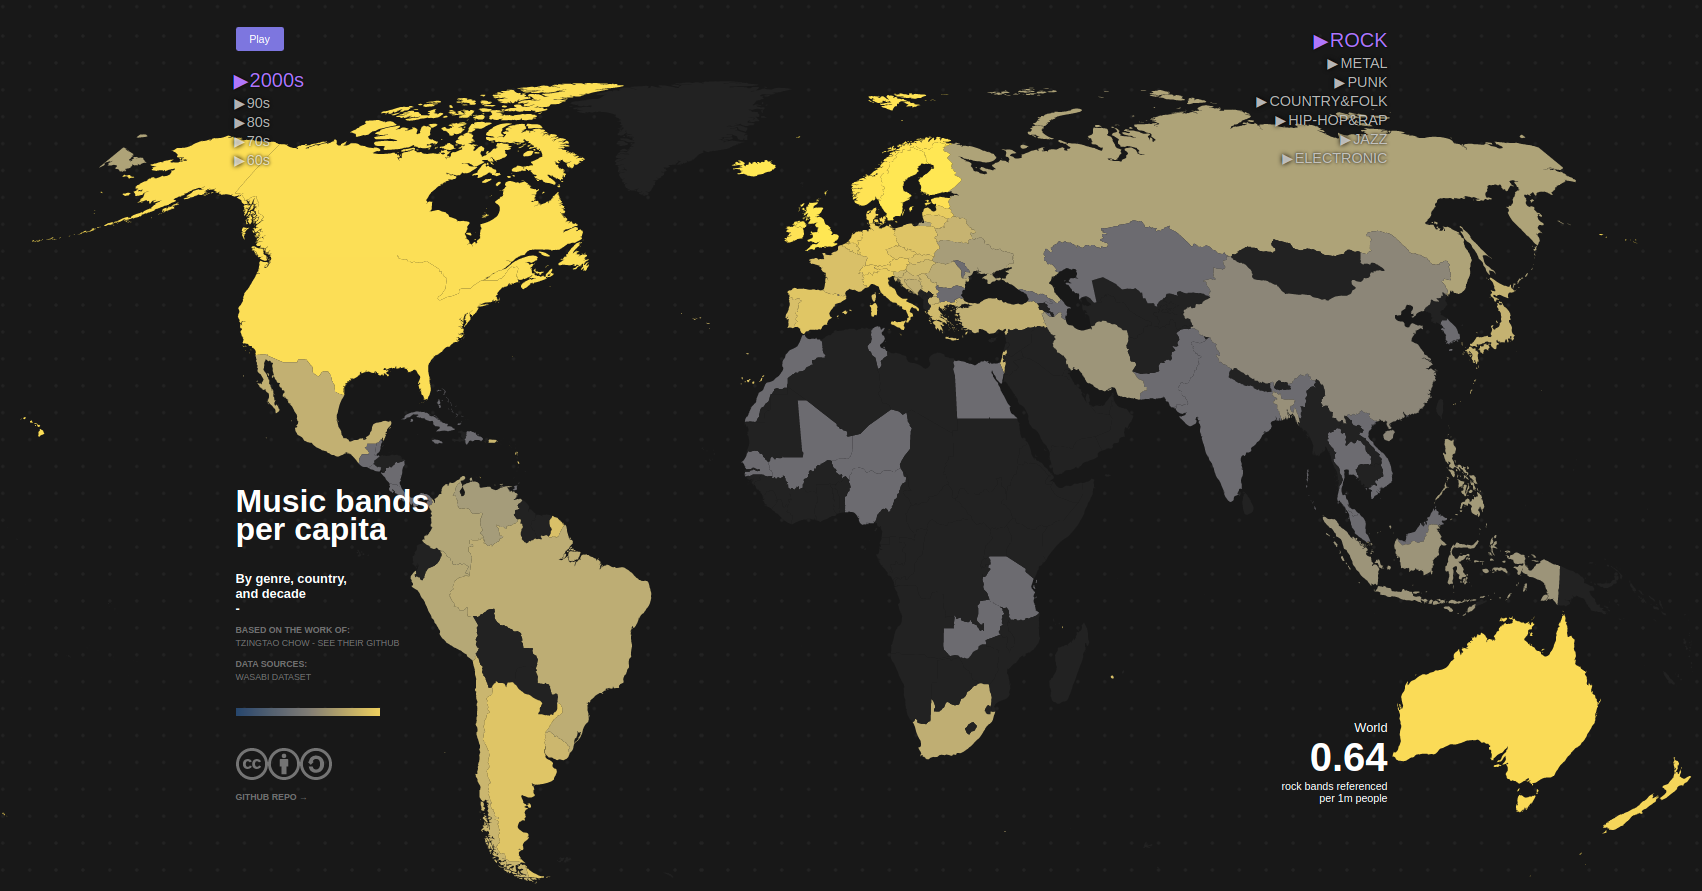
\includegraphics[width=0.98\linewidth]{map.png}
    \caption{Choropleth Map implementation\label{fig:a}}
    \end{figure}
    
    \section*{Evaluation Format}

    This document must not be shared with the participants as before-hand knowledge of the application is not permitted. The goal is to avoid preparedness to the task.
    \newline
    \newline
    The evaluation process is structured in three steps:
    \begin{itemize}
        \item Welcoming, briefing, and interview of the participants (with a questionnaire)
        \item The participants discover the application and must go through a series of monitored tasks
        \item Debriefing and interview of the participants (questionnaire and end survey)
    \end{itemize}

    \subsection*{Participant-Oriented Evaluation Method}
    
    We choose a participant-oriented method with the following question as our driver: 
    
    \begin{quote}
        Can a participant complete a set of increasingly demanding tasks on a data visualization format they have never encountered before?
    \end{quote}
    
    We focus on efficiency (i.e. how quickly a participant can achieve a task) and participant satisfaction.

    \subsection*{Hypothesis Regarding The Data Visualization Format}
 
    The experimental design is not duplicated between various forms of UI or between different conditions. As such, there are no hypothesis associated with the current implementation of a data visualization.
 
    \subsection*{Metrics}
    
    To measure the participants' handling of their tasks, the following metrics are considered:
    
    \begin{itemize}
        \item For effectiveness: 
        \begin{itemize}
            \item Number of successful task completions
            \item Number of clicks performed to achieve a task compared to the minimum achievable
            \item Tracking of eye movements
            \item Tracking of mouse pointer movements
        \end{itemize}
        \item For satisfaction: end-questionnaire to assess usability (e.g. SUS)
    \end{itemize}
    
    \section*{Test Session Checklist}
    A session corresponds to running a single participant through the whole process from start to finish, unless a stopping event is reached. Any session \textit{must} follow the following steps:
    \begin{itemize}
        \item Welcoming the participant and introducing them to each involved party: the tester/observer, etc.
        \item \textit{Each of the following steps must be preceded with asking the participant if they have any questions, are comfortable, and wish to proceed}
        \item Introducing the participant to:
        \begin{itemize}
            \item the \textbf{evaluation process}: reason(s) for evaluating participants on the future task, goals of compiling their data (see Annex 1)
            \item the \textbf{context}: They will be tested on a Data Visualization application (see Annex 2)
            \item the \textbf{place}: the testing area
            \item the \textbf{hardware setup}, e.g., computer monitor (output to the participant), mouse (input from the participant), the means of observation of the participant and (mouse tracker, camera, etc.)
        \end{itemize}
        \item Have the participant sign all required disclosure agreements or letters of understanding (see Annex 3)
        \item Have the participant answer a profile questionnaire before starting the tasks (see Annex 4)
        \item The tester/observer removes themselves from the test area, and mentioned to the participant they can start
        \item The participant reveals their instructions and proceeds (see Annex 5)
        \item Once each task is performed, the tester/observer comes back to the test area
        \item Have the participant answer a system usability survey (see Fig. 1, and Annex 6) and a post-task questionnaire (see Annex 7)
        \item Thank the participant as they leave
    \end{itemize}
    
    \section*{Pre-Task Questionnaire}
    
    During the first part of the test, and after a disclosure agreement/letter of understanding has been signed (see Annex 3), the participant is invited to complete a questionnaire split in two parts (see Annex 4):
    \begin{itemize}
        \item \textbf{Participant info}: Name, contact information, etc. which make the participant reachable
        \item \textbf{Participant prior experience} (meant to help size the participant's profile)
        % \begin{itemize}
        %     \item Do you play a music instrument? [Y]/[N]
        %     \item Are you subscribed to an audio streaming platform? [Y]/[N]
        %     \item How many hours per week do you dedicate to listening to music? [less than 1 hour]/[1 to 5h]/[6 to 10h]/[More than 10 hours]
        %     \item How many music genres do you say you mainly listen to? [1]/[2]/[3]/[More than 3]
        %     \item Do you read or follow (on social media) music bands or news media dedicated to music (e.g. Rolling Stones magazine)? [Y]/[N]
        % \end{itemize}
    \end{itemize}
    
    \section*{Tasks}
    
    Once the pre-task questionnaire is filled and the participant is ready to continue, they are given a series of tasks to perform (see Annex 5 for the exhaustive list of tasks for the project). Each task is formatted as follow:
    \begin{itemize}
        \item Task description
        \item Evaluation question from the participant's perspective (e.g. how hard they found the task)
        \item Open-ended question for the participant on how they would improve the question
    \end{itemize}
    
    \begin{figure}	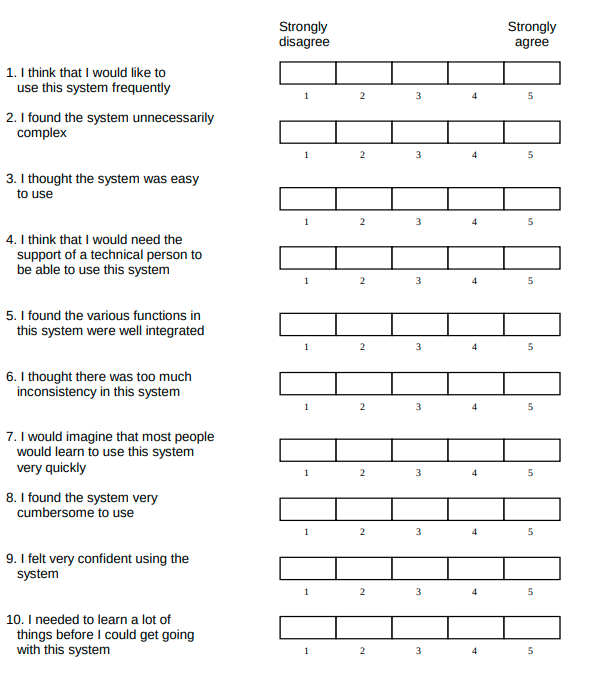
\includegraphics[width=0.98\linewidth]{SUS.png}
    \caption{Original System Usability Scale questionnaire\label{fig:b}}
    \end{figure}

    \section*{System Usability Scale survey}
    
    Once the tasks have been completed or attempted, the participant is given a post-task survey. The one used in this project follows the \textbf{System Usability Scale} standard (see Fig. \ref{fig:b}) from J. Brooke\cite{brook}. It is a standard questionnaire used for assessing the overall usability of a system/tool/etc. Based on the contained 10 standard questions (see Annex 6), it allows to calculate a score from 0 to 100 (from worst to best) to inform testers/observers of the overall usability and efficient learning of a system/tool/etc. by a novice user.
    
    \section*{End Questionnaire}
    
    Once the survey is completed, a final questionnaire is provided to the participant (see Annex 7).

    \section*{Data Visualization Results}
    
    \textbf{Based on a preliminary run through a single person, the application yielded a SUS score of 85 out of 100}. Overall, the test participant found the application easy to navigate, finding difficulties not in the tool but the way the evaluation was organized -- notably that the questions were asked by voice rather than printed on paper.
    
    The main criticism the application received was related to the color scale of a genre ("Jazz") which was not sharp enough. The second criticism is related to the zoom function which is reset every time the user changes a parameter.  
    
    \section*{Annex 0 - Shape of the Choropleth map}

    \section*{Annex 1 - Introduction to the Choropleth evaluation}
    
    \begin{quote}
        "Welcome, my name is [tester/observer]. We are going to walk you through today's session. It should take between twenty and thirty minutes of your time. Our purpose is to evaluate the usability and engagement of participants towards a newly developed Data Visualization tool. This tool will allow you to explore data related to music genres across the world and decades.
        \newline\newline
        Before we proceed, we want to thank you for clearing your time schedule for us. Your input is valuable for our research and will help up determine the current state of our development and where to improve the tool."
    \end{quote}
    
    \section*{Annex 2 - Statement of purpose for the Choropleth evaluation}
    
    \begin{quote}
        "This session is organized in a few steps, the first of which is asking you to review a document called a 'Letter of Understanding' that will describe the goal of your participation. If you agree to it and sign it -- it works as consent --, we will then proceed with a questionnaire that will ask you about your demographics and background. Once filled, we will ask you to take seat in front of a computer and follow a series of tasks to accomplish on an application that will be displayed on a monitor. The application itself is displayed inside a web browser such as Internet Explorer or Google Chrome. You will be given a mouse and keyboard to perform those tasks. 
        \newline\newline
        While performing those tasks, your reactions and movements will be recorded to assess your primary reaction to the application. Please note that there are no wrong ways to arrive an an answer. As you are performing the task, we will ask you to speak out loud your thought process and remarks as often as possible. The goal is to capture your thought process, what you are looking at, what you are trying to do. This is a tremendous help for our research.
        \newline\newline
        You can ask us any question at any time as you continue through the process. We may not be able to provide an answer right away as we are interested in your reaction in a seemingly unsupervised manner.
        \newline\newline
        After you are done with the tasks, or after you stop the process, we will go proceed to a final interview where you will be asked a survey about the application you just used, and finally a questionnaire about your general comprehension of the tool and process involved."
    \end{quote}
    
    \section*{Annex 3 - Letter of Understanding/Disclosure Agreement for the Choropleth evaluation}
    
    \begin{quote}
        "\textit{Please read this page carefully}
        \newline\newline
        By Participating in this evaluation, you will be assessed to help our program improve a data visualization tool related to the evolution of music data across the world and past decades. You will be observed and the way you interact with the application will be collected. You will also be asked to fill out 2 questionnaires, 1 survey, and answer interview questions if need be.
        \newline\newline
        By signing the present form, you give your permission for your data (verbal statements, computer inputs such as mouse movements, visual data such as eye movements, etc.) to be collected for the purpose of evaluating, improving, and displaying the application. Your personal identifiable data such as your name will not be used.
        \newline\newline
        You can withdraw from this test at any time and unilaterally. You may ask any question at any time.
        \newline\newline
        If you agree with these terms, please indicate your agreement by providing your name, signature, and current date."
    \end{quote}
    
    \section*{Annex 4 - Profile questionnaire for the Choropleth evaluation}
    
    \begin{itemize}
        \item Personal Information:
        \begin{itemize}
            \item Name, Age, \& Email 
            \item Gender (Male, Female, Other)
            \item Education Level (None, High School, Undergrad, Graduate, PhD)
            \item Current Occupation (Student, Employee, etc.)
        \end{itemize}
        \item Participant's Profile Information:
        \begin{itemize}
            \item Do you play a music instrument? [Yes/No]
            \item Are you subscribed to an audio streaming platform (e.g. Spotify)? [Yes/No]
            \item How many hours per week do you dedicate to listening to music? [<1h, 1-3h, 3h+]
            \item How many music genres do you mainly listen to? [1, 2, 3+]
            \item Do you read or follow (on social media) music bands or music-dedicated news media? [Yes/No]
            \item Do you know what a Choropleth map is? [Yes/No]
            \item On a scale of 1 (least) to 5 (very), how easy was it to answer the questions above? [1-5]
        \end{itemize}
    \end{itemize}
    
    \section*{Annex 5 - Choropleth evaluation tasks}
    
    \subsection*{Training Explanation}
    
    \begin{quote}
        "You have been given a Choropleth map: a visual representation of the density of an occurrence across a region. 
        \newline\newline
        Here you are able to explore the number of bands available in the WASABI dataset per country, per capita, per decade, and per genre across the world (You can select any decade since the 1960s and any of seven main genres, and select/hover on any country, to display the related data). 
        \newline\newline
        The color gradient represents the concentration of bands in a country.
        \newline\newline
        Please find below a series of tasks to complete. you may stop at any time. Please remember to think out loud whenever possible to walk us through your mental process. Good luck!"
    \end{quote}
    
    \subsection*{Tasks}
    
    \begin{center}
    \begin{tabular} { | c | l | c | }
    \hline
     Task & Description & Metrics \\
    \hline
    \textbf{1} & You have entered a new & \# of clicks \\
    & website displaying a & Time spent\\
    & world map. Find the & Eye moves\\
    & average population for & Mouse moves\\
    & the United States of & \\
    & America in in the 2000s.& \\
    \hline
    Q1. & How easy was & 1 to 5\\
    & it to find the value? & scale \\
    \hline
    Q2 & What would you change to & open\\
    & make the process easier? & question\\
    \hline
    \end{tabular}
    \end{center}

    \begin{center}
    \begin{tabular} { | c | l | c | }
    \hline
     Task & Description & Metrics \\
    \hline
    \textbf{2} & Find the number of & \# of clicks \\
    & rock bands in the United & Time spent\\
    & States in the 1980s. & Eye moves\\
    &  & Mouse moves\\
    \hline
    Q1. & How easy was & 1 to 5\\
    & it to find the value? & scale \\
    \hline
    Q2 & What would you change to & open\\
    & make the process easier? & question\\
    \hline
    \end{tabular}
    \end{center}
    
    \begin{center}
    \begin{tabular} { | c | l | c | }
    \hline
     Task & Description & Metrics \\
    \hline
    \textbf{3} & Find the ratio of rock & \# of clicks \\
    & bands per one million & Time spent\\
    & people in the United & Eye moves\\
    & States in the 1960s. & Mouse moves\\
    \hline
    Q1. & How easy was & 1 to 5\\
    & it to find the value? & scale \\
    \hline
    Q2 & What would you change to & open\\
    & make the process easier? & question\\
    \hline
    \end{tabular}
    \end{center}
    
    \begin{center}
    \begin{tabular} { | c | l | c | }
    \hline
     Task & Description & Metrics \\
    \hline
    \textbf{4} & Find the ratio of electro & \# of clicks \\
    & bands in Germany in the & Time spent\\
    & 1990s. & Eye moves \\
    & & Mouse moves \\
    \hline
    Q1. & How easy was & 1 to 5\\
    & it to find the value? & scale \\
    \hline
    Q2 & What would you change to & open\\
    & make the process easier? & question\\
    \hline
    \end{tabular}
    \end{center}

    \begin{center}
    \begin{tabular} { | c | l | c | }
    \hline
     Task & Description & Metrics \\
    \hline
    \textbf{5} & Find the percentage share & \# of clicks \\
    & of hip-hop bands over the & Time spent\\
    & total number of bands in & Eye moves\\
    & France in the 1990s. & Mouse moves\\
    \hline
    Q1. & How easy was & 1 to 5\\
    & it to find the value? & scale \\
    \hline
    Q2 & What would you change to & open\\
    & make the process easier? & question\\
    \hline
    \end{tabular}
    \end{center}
    
    \begin{center}
    \begin{tabular} { | c | l | c | }
    \hline
     Task & Description & Metrics \\
    \hline
    \textbf{6} & Find whether Andorra (a & \# of clicks \\
    & small country between & Time spent\\
    & France and Spain) had & Eye moves\\
    & metal bands in the 2000s.  & Mouse moves\\
    \hline
    Q1. & How easy was & 1 to 5\\
    & it to find the value? & scale \\
    \hline
    Q2 & What would you change to & open\\
    & make the process easier? & question\\
    \hline
    \end{tabular}
    \end{center}

    \begin{center}
    \begin{tabular} { | c | l | c | }
    \hline
     Task & Description & Metrics \\
    \hline
    \textbf{7} & Find which country had & \# of clicks \\
    & the highest ratio of jazz & Time spent\\
    & band per capita in the & Eye moves\\
    & world in the 2000s. & Mouse moves\\
    \hline
    Q1. & How easy was & 1 to 5\\
    & it to find the value? & scale \\
    \hline
    Q2 & What would you change to & open\\
    & make the process easier? & question\\
    \hline
    \end{tabular}
    \end{center}
    
    \begin{center}
    \begin{tabular} { | c | l | c | }
    \hline
     Task & Description & Metrics \\
    \hline
    \textbf{8} & Automatically play the & \# of clicks \\
    & sequence of map per & Time spent\\
    & decade for the genre & Eye moves\\
    & Punk. & Mouse moves\\
    \hline
    Q1. & How easy was & 1 to 5\\
    & it to find the value? & scale \\
    \hline
    Q2 & What would you change to & open\\
    & make the process easier? & question\\
    \hline
    \end{tabular}
    \end{center}
    
    \section*{Annex 6 - SUS survey of the Choropleth evaluation} 
    
    Each item of the survey is rated from 1 (strongly disagree) to 5 (strongly agree).
    
    \begin{itemize}
        \item I think that I would like to use this type of data visualization more frequently
        \item I found this type of data visualization unnecessarily complex
        \item I thought the Choropleth map was easy to use
        \item I think that I would need the support of a technical person to be able to use such a map
        \item I found the various way to display information on the map were well integrated
        \item I thought there was too much inconsistency on the map
        \item I would imagine that most people would learn to use this type of visualization very quickly
        \item I found the map very cumbersome to use
        \item I felt very confident in navigating the map
        \item I needed to learn a lot of things before I could get going with this system
    \end{itemize}

    \section*{Annex 7 - Final questionnaire of the Choropleth evaluation} 
    
    \begin{itemize}
        \item What did you like and/or dislike about the evaluation process?
        \item Have you had any difficulties, if so where?
        \item For each task, were you confident beforehand that your interaction with the application would output the right results?
        \item What would you change to the data visualization application?
        \item What would you change to the evaluation process?
        \item Please describe in one sentence the data visualization application you used?
    \end{itemize}
    
    \section*{Annex 8 - Example participant feedback for the Choropleth evaluation} 
    
    \subsection*{Pre-Task Questionnaire}
    \begin{itemize}
        \item Personal Information: 
        \begin{itemize}
            \item \textbf{Name}: C*****s C********o
            \item \textbf{Email}: c*********o@yahoo.fr
            \item \textbf{Gender}: Male
            \item \textbf{Age}: 23
            \item \textbf{Education Level}: Undergrad
            \item \textbf{Current Occupation}: Student 
        \end{itemize}
        \item Participant's Profile Information
        \begin{itemize}
            \item Do you play a music instrument? \textbf{No}
            \item Are you subscribed to an audio streaming platform (e.g. Spotify)? \textbf{Yes}
            \item How many hours per week do you dedicate to listening to music? \textbf{1-3h}
            \item How many music genres do you mainly listen to? \textbf{3+}
            \item Do you read or follow (on social media) music bands or music-dedicated news media? \textbf{No}
            \item Do you know what a Choropleth map is? \textbf{Yes}
            \item On a scale of 1 (least) to 5 (very), how easy was it to answer the questions above? \textbf{5}
        \end{itemize}
    \end{itemize}
    
    \subsection*{Tasks}
    \begin{itemize}
        \item \textbf{Task 1}:
        \begin{itemize}
            \item Was the task achieved? \textbf{Yes}
            \item Easiness Rating by Participant (1-hardest to 5-easiest): \textbf{5}
            \item Did the participant offer to change something? \textbf{No}
        \end{itemize}
        \item \textbf{Task 2}:
        \begin{itemize}
            \item Was the task achieved? \textbf{Yes}
            \item Easiness Rating by Participant (1-hardest to 5-easiest): \textbf{5}
            \item Did the participant offer to change something? \textbf{No}
        \end{itemize}
        \item \textbf{Task 3}:
        \begin{itemize}
            \item Was the task achieved? \textbf{Yes}
            \item Easiness Rating by Participant (1-hardest to 5-easiest): \textbf{4}
            \item Did the participant offer to change something? \textbf{Yes}, maybe include the ratio in the tooltip.
        \end{itemize}
        \item \textbf{Task 4}:
        \begin{itemize}
            \item Was the task achieved? \textbf{Yes}
            \item Easiness Rating by Participant (1-hardest to 5-easiest): \textbf{5}
            \item Did the participant offer to change something? \textbf{No}
        \end{itemize}
        \item \textbf{Task 5}:
        \begin{itemize}
            \item Was the task achieved? \textbf{Yes}
            \item Easiness Rating by Participant (1-hardest to 5-easiest): \textbf{4}
            \item Did the participant offer to change something? \textbf{Yes}, maybe provide more information on what the ratio mean.
        \end{itemize}
        \item \textbf{Task 6}:
        \begin{itemize}
            \item Was the task achieved? \textbf{Yes}
            \item Easiness Rating by Participant (1-hardest to 5-easiest): \textbf{3}
            \item Did the participant offer to change something? \textbf{Yes}, remove automatic unzooming
        \end{itemize}
        \item \textbf{Task 7}:
        \begin{itemize}
            \item Was the task achieved? \textbf{Yes}
            \item Easiness Rating by Participant (1-hardest to 5-easiest): \textbf{3}
            \item Did the participant offer to change something? \textbf{Yes}, spread the range of color for Jazz
        \end{itemize}
        \item \textbf{Task 8}:
        \begin{itemize}
            \item Was the task achieved? \textbf{Yes}
            \item Easiness Rating by Participant (1-hardest to 5-easiest): \textbf{5}
            \item Did the participant offer to change something? \textbf{No}
        \end{itemize}
    \end{itemize}
    
    \subsection*{SUS Survey}
    \begin{itemize}
        \item I think that I would like to use this type of data visualization more frequently | 2
        \item I found this type of data visualization unnecessarily complex | 2
        \item I thought the Choropleth map was easy to use | 5
        \item I think that I would need the support of a technical person to be able to use such a map | 1
        \item I found the various way to display information on the map were well integrated | %
        \item I thought there was too much inconsistency on the map | 1
        \item I would imagine that most people would learn to use this type of visualization very quickly | 5
        \item I found the map very cumbersome to use | 2
        \item I felt very confident in navigating the map | 4
        \item I needed to learn a lot of things before I could get going with this system | 1
    \end{itemize}
    
    \textit{To calculate the SUS score, first sum the score contributions from each item. Each item's score contribution will range from 0 to 4. For items 1,3,5,7,and 9 the score contribution is the scale position minus 1. For items 2,4,6,8 and 10, the contribution is 5 minus the scale position. Multiply the sum of the scores by 2.5 to obtain the overall value of SU}.
    \newline\newline
    The total score is: \textbf{85} out of 100.
    
    \subsection*{End Questionnaire}
    \begin{itemize}
        \item What did you like and/or dislike about the evaluation process? \textbf{Questions were asked via voice. Providing a paper version would be better for people who are not English native speakers}.
        \item Have you had any difficulties, if so where? \textbf{No}.
        \item For each task, were you confident beforehand that your interaction with the application would output the right results? \textbf{Most of the time}.
        \item What would you change to the data visualization application? \textbf{Some color scales could be made more pronounced}. 
        \item What would you change to the evaluation process? \textbf{Nothing}.
        \item Please describe in one sentence the data visualization application you used? \textbf{Evolution of music genres by decade}.
    \end{itemize}
    
    \bibliographystyle{unsrtnat}   
    \begin{thebibliography}{9}

    \bibitem{brook}
    Brooke, John. (1995). \textit{\href{https://hell.meiert.org/core/pdf/sus.pdf}{SUS: A quick and dirty usability scale}}. Usability Eval. Ind.. 189. 

    \end{thebibliography}
    
\end{document}